%! Author = t.kramer
%! Date = 15/09/2024

\section{Research context}

% Context
Indoor thermal comfort is strongly associated with occupant well-being \citep{altomonte_ten_2020}, overall satisfaction \citep{graham_lessons_2021}, and energy use in buildings \citep{yang_thermal_2014}. As such, accurately projecting operational thermal comfort is a critical aspect of building design.

% Workflow: where do we use metrics + what are common examples
In traditional design workflows, thermal comfort assessments rely heavily on simulation data. Typically, these data points form the basis for calculating hourly thermal comfort indices, e.g., the Predicted Mean Vote (PMV), which are then aggregated into a single-value annual metric (see \Cref{fig:typical-workflow}). Common long-term metrics based on this approach include the \textit{Percentage of Time Outside a PMV Range} and the \textit{Percentage of Time Outside an Operative Temperature Range}, both featured in ISO-7730, EN-16798, and ASHRAE-55 \citep{iso_2005, cen_en_2019, ashrae_2023}. Other measures adopted by global standards are the \textit{Degree Hours} (ISO-7730, EN-16798) or the \textit{Average PPD} \citep{iso_2005} methods. 


\begin{figure*}[h!]
    \centering
    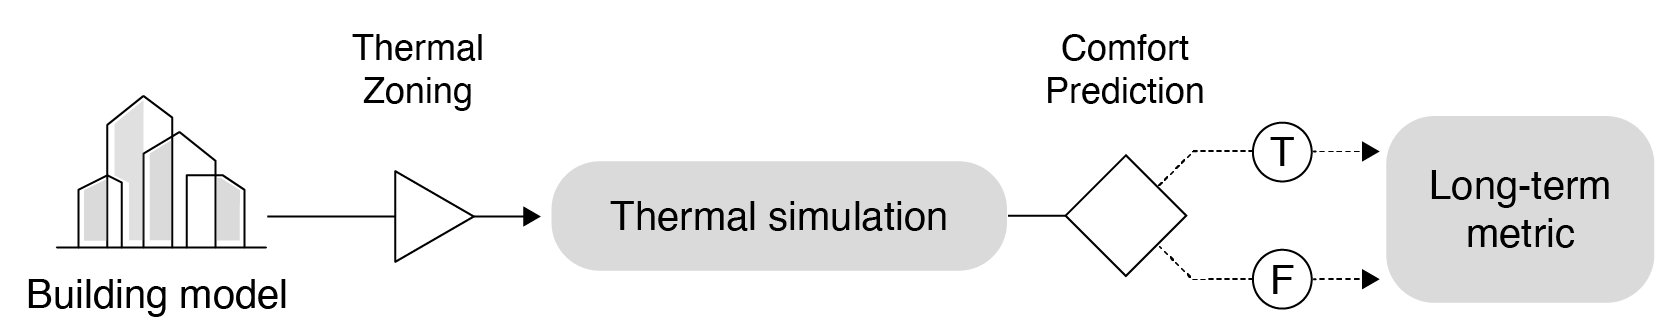
\includegraphics[width=\textwidth]{manuscript/src/figures/workflow-black-short.png}
    \caption{Traditional long-term thermal comfort prediction: The building model is divided into thermal zones and simulated in hourly time steps; simulated indoor climate data is then assessed using a thermal comfort index (e.g., PMV or operative temperature) and aggregated into a single-value long-term (e.g., annual or seasonal) metric. }
    \label{fig:typical-workflow}
\end{figure*}


% the most frequently used metrics rely on the Predicted Mean Vote (PMV) or Predicted Percentage Dissatisfied (PPD) models. Recent research has highlighted several problems of the PMV index: it often exhibits poor predictive accuracy \citep{cheung_analysis_2019}, advocates for excessively narrow temperature ranges \citep{arens_are_2010}, and is highly sensitive to personal input parameters such as clothing insulation and metabolic activity \citep{gauthier_role_2013}—variables that are hard to predict and often treated as constants in models \citep{carlucci_review_2012}, thus failing to represent real-world behavior accurately. Overall, these limitations tend to promote overly tight temperature ranges, which in turn leads to excessive energy use for space conditioning \citep{albatayneh_impact_2018, fukawa_field_2021, sekhar_thermal_2016}.

Beyond the commonly used metrics found in building standards, research has introduced several alternative approaches. For example, based on continuous monitoring and post-occupancy evaluations in air-conditioned offices, \citet{li_improved_2020} identified the percentage of time the daily temperature range exceeded a set threshold as a particularly effective index. This concept of temporal exceedance has also been explored by others \citep{borgeson_comfort_2011, nicol_suggestion_2009}. Additional recommendations include evaluating the fraction of time within adaptive comfort limits \citep{albatayneh_development_2019}, using adaptive degree days \citep{mcgilligan_adaptive_2011}, and tracking overheating degree-days \citep{estrella_guillen_comparing_2019}. In general, these metrics provide a broad annual assessment of thermal comfort and are instrumental in guiding key design decisions regarding the building's form and envelope, and in the design and sizing of HVAC systems.

% BUT
However, despite the widespread adoption of standard thermal comfort workflows and metrics and continued research activity on identifying novel metrics, all presented methods share one substantial limitation, they typically capture only the temporal variability of thermal comfort while overlooking spatial differences within a thermal zone. This is a significant oversight, as is has been highlighted in \citep{mishra_thermal_2016, kramer_personal_2023}.

% Objective  
We aim to introduce a new metric for the evaluation of building performance based on comfort: spatial thermal autonomy (sTA). Compared to traditional metrics, sTA offers two significant advantages: (a) it accounts for spatial thermal variability, ensuring a more comprehensive evaluation of comfort throughout a building, and (b) it quantifies how much a building is able to provide thermally comfortable conditions without the use of active sources of energy.




